\documentclass{article}
\usepackage[utf8]{inputenc}
\usepackage[margin=1in]{geometry}
\usepackage{mathtools,setspace,indentfirst,graphicx,float,url,color}
\usepackage{fancyhdr} % for header
\usepackage{listings}
\usepackage[english]{babel}
\usepackage[backend=biber,style=numeric]{biblatex}
\addbibresource{sources.bib}

\doublespacing{}

\fancyhf{}
\pagestyle{fancy}

\lhead{N Batista, M Inciong, F Truncale}
\chead{\thepage}
\rhead{Fall 2017}
\renewcommand{\headrulewidth}{0pt} % remove the horizontal line along the header

\lstset{%
  basicstyle=\ttfamily,
  captionpos=b,
  frame=tb,
  tabsize=2,
  showstringspaces=false,
  commentstyle=\color[RGB]{24,135,64},
  keywordstyle=\color{blue},
  stringstyle=\color{red}
}

\begin{document}

\thispagestyle{empty}

\begin{titlepage}
  \vspace*{\fill} % i copied this off stackexchange so no i don't know what that asterisk does.
  \begin{center}
    {\Huge Milestone Report --- Optimization of Subgraph Isomorphism Algorithm}\\[0.4cm]
    {\huge by Nelson Batista, Max Inciong, Francesca Truncale}\\[0.5cm]
    {\huge Senior Project II}\\[0.4cm]
    {\huge Professor Jianting Zhang}\\[0.4cm]
    {\LARGE Fall 2017}
  \end{center}
  \vspace*{\fill}
\end{titlepage}

\pagenumbering{roman}
%table of contents
\tableofcontents

\newpage

\pagenumbering{arabic}
\setcounter{page}{1}

%\addcontentsline{toc}{section}{Introduction}
\section{Introduction}

The goal of this project is to understand and optimize an algorithm for solving the NP-complete problem of subgraph isomorphism. 

  \subsection{Background}

  An \textit{isomorphism} between two graphs is a mapping from the vertices of one graph, say $G$, to another graph, say $H$, such that any two vertices which are adjacent in $G$ are mapped to vertices which are adjacent in $H$. The subgraph isomorphism problem, in turn, is the problem of determining whether an isomorphism exists between a graph $G$ and any of the subgraphs of a larger search graph, $H$. The issue that makes the subgraph isomorphism problem so difficult to solve for a particular pair of graphs is cycling through the main graph and expanding each node within the graph and checking if each of the generated subgraphs formed from each node is isomorphic to the control graph.

  Fortunately, many attempts exist to solve the subgraph isomorphism problem. Among the earliest of these is the famous \textit{Ullmann Algorithm}, proposed by Julian R. Ullmann in his 1976 paper, \textit{An Algorithm for Subgraph Isomorphism}. He first describes a basic, naive approach to finding a mapping from the vertices of a graph to a subgraph of a larger graph. He goes on to define a ``refine'' procedure to dramatically reduce the number of possible mappings that must be checked.\cite{ullmann} These will be covered in greater detail in the next section.

  The goal of our project was to take this algorithm and improve its performance. Subgraph isomorphism is an expensive problem to solve, and finding multiple possible isomorphisms from one graph to subgraphs of another is even more expensive, so even slight improvements in the algorithm's performance is likely to lead to large performance improvements in any large-scale program which needs to use it often.

  \subsection{Motivation}

  Our reasoning for choosing this topic for our project is an apparent lack of especially efficient algorithms for solving the subgraph isomorphism problem. Solutions to the subgraph isomorphism problem are often used to detect similarities in chemical compounds,\cite{ullmann} which may shed light on some of their properties. If this process needs to be done, for example, on a very large database of chemical compounds, or less frequently for several very large compounds, the process may take a very long time to complete. It would be very beneficial to improve the performance of this algorithm, even if only slightly, so that these sorts of use cases can still be handled in a more reasonable amount of time.

  \subsection{Data Set}

  The primary graph used to test the algorithm and its performance is an undirected graph consisting of ``friends lists'' from the social media website, Facebook. Each node of the graph represents a unique user, and, if two nodes are adjacent, then their corresponding users are friends on Facebook.\cite{fbgraph} 
  
  The graph contains 4,039 nodes and 88,234 edges. The relatively large size of the graph makes it well-suited to use for collection of performance data. As we shall see, the Ullmann algorithm takes a rather long time to complete with a graph of this size, allowing any optimizations and/or parallelizations to be readily apparent.

\section{Ullmann Algorithm}

  \subsection{Naive Approach}

  The paper begins, as many do, with a definition of terms that will be used throughout. We have repeated them here for the sake of clarity later on. We begin by noting that the algorithm models the search for a possible mapping by having all possible mappings as nodes on a tree, on which a depth-first search is performed to find a solution.

  The subgraph isomorphism problem is defined as the problem of finding all isomorphisms between a graph $G_\alpha = (V_\alpha, E_\alpha)$ and subgraphs of another graph $G_\beta = (V_\beta, E_\beta)$, with $(V_\alpha, E_\alpha)$ and $(V_\beta, E_\beta)$ being the set of vertices and edges of $G_\alpha$ and $G_\beta$, respectively. The number of vertices and edges of $G_\alpha$ and $G_\beta$, respectively, are $(p_\alpha, q_\alpha)$ and $(p_\beta, q_\beta)$.

  The \textit{adjacency matrix} for graph $G_\alpha$, $[a_{ij}]$, is defined by:

  \[ a_{ij} = \begin{cases}
                1 & \textrm{ if } i \neq j \textrm{ and } i,j \textrm{ share an edge} \\
                0 & \textrm{ otherwise} 
  \end{cases}
  \]

  The adjacency matrix for graph $G_\beta$, $[b_{ij}]$, is defined equivalently.

  Notably, we have the $p_\alpha \times p_\beta$ matrix $M$, which is a binary matrix of assignments (mappings) from $V_\alpha$ to $V_\beta$. That is, if $m_{ij}$ is 1, then vertex $i$ in graph $G_\alpha$ could possibly be mapped to vertex $j$ in $G_\beta$. Otherwise $m_{ij}$ is 0. M has a few interesting properties as a result, which will soon be apparent. 

  Finally, we come to $d$, which is simply algorithm's current depth in the search tree. The algorithm starts at $d = 0$, and terminates when $d = p_\alpha$. The matrix $M$ at a particular depth $d$ is denoted as $M_d$, with solutions to the working instance of the subgraph isomorphism problem being the set of assignments from $V_\alpha$ to $V_\beta$, contained within matrices $M_{p_\alpha}$. $M_0$ is generated by the following formula:

  \[ m_{ij} = \begin{cases}
    1 & \textrm{ if degree} (j \in G_\beta) \geq \textrm{ degree} (i \in G_\alpha) \\
                0 & \textrm{ otherwise} 
  \end{cases}
  \]

  Each step of the computation consists of setting all but one of the values of one of the rows of $M$ to 0, and then checking whether exactly one 1 exists in each row.
  We also have a $p_\beta$-bit binary vector $\vec{F}$. $\vec{F}_i$ is 1 if column $i$ of matrix $M$ has been used so far in the computation. We also have vector $\vec{H}$, with $\vec{H}_d = k$ if column $k$ of matrix $M$ was used at depth $d$, and 0 otherwise.
  In the most basic algorithm, the entire tree is searched, including branches which cannot possibly contain a solution at any depth. The algorithm is below:
  
  \begin{enumerate}
    \item $M=M_0$, $d=0$, $H_0 = 0$, set all $F_i$ to 0.

    \item
  \end{enumerate}

  \subsection{``Refine M'' Procedure}

  \subsection{Full Algorithm}

\section{Implementation of the Algorithm}

The full source code for all versions can be found in the appendix.

  \subsection{Python Implementation}
  The Python code is based largely on an implementation of the Ullmann algorithm provided by an answer on the website \textit{StackOverflow}.\cite{pyiso} It would not run in its original form, so a few adjustments were needed.

  \begin{lstlisting}[language=Python,caption={Function used to determine whether an isomorphism exists.}]
  def find_isomorphism(graph, subgraph):

      assignments = []
      possible_assignments = [[True]*graph.n_vertices() \
                    for i in range(subgraph.n_vertices())]
      if search(graph, subgraph, assignments, possible_assignments):
          return True
      return matches
  \end{lstlisting}

  The main function is \texttt{find\_isomorphism}, which is depicted above. It calls the function \texttt{search}, which performs the actual work of finding an isomorphism.

  The \texttt{search} function runs  the \texttt{update\_possible\_assignments} function. This particular function has been the subject of refining over the course of the project. At the time of the python implementation, it was the most significant bottleneck.

  This was mostly due to the usage of the \texttt{has\_edge} method of the graph class, shown below.

  \begin{lstlisting}[language=Python,caption={Code for the \texttt{has\_edge} method of our graph class.}]
  def has_edge(self, vert1, vert2):
       """ Checks if edge connecting vert1 and vert2 is in the graph
       """
       #if adjacent, there's an edge
       return ({vert1, vert2} in self.adjacencies) 

  \end{lstlisting}

  This method calls the built-in \texttt{in} function of Python lists, which has a runtime complexity of O(n).\cite{bigopy} Thus, the \texttt{has\_edge} method of the Python implementation is O(n).

  \subsection{Initial C++ Implementation}

  The initial C++ implementation was based entirely on the Python implementation. Indeed, it represented our best attempt to ``translate'' the Python code to C++. As one might imagine, it was riddled with compilation errors. That said, we did manage to get it to run, and analysis indicated it performed little better than the Python equivalent. We suspected this was because it retained the same issue that the Python implementation had: calling \texttt{has\_edge}, an O(n) method, countless times. This motivated a significant improvement.

  \subsection{Improved C++ Implementation}

  The improved C++ implementation represents a significant milestone in our project, as it not only improved upon the clarity of the isomorphism algorithm, but also resulted in a much cleaner graph class, with edges implemented as an adjacency matrix. This makes the \texttt{has\_edge} function O(1), as it consists of simply looking up whether the given vertices share an edge by checking the matrix. This makes its repeated use in \texttt{refine\_possible\_assignments} much more acceptable, a fact which is reflected in the performance.

  We also have stored vertices in such a way that each vertex is also stored along with its degree, allowing quick and easy lookup of a vertex's degree.

  \subsection{Optimizations through OpenMP}
  OpenMP utilizes the multiple cores of a computer's processor in order implement multithreading to run related tasks in parallel. We intend to use it where the bottlenecks in our algorithm are to improve the algorithm's performance. The default number of cores for many computers is four. We intend to place the parallelisms where there tend to be a large number iterations, specifically in loops. This means that, theoretically, the program should run four times faster than without multithreading, using our earlier assumption of four processor cores allotted to the algorithm. It is more likely that it will be approximately 3 to 3.5 times faster, since we may not be able to completely parallelize the bottlenecks as intended. Additionally, using OpenMP, as is the case with any parallelization method, comes with a certain amount of overhead in separating the work to be done. There is also the issue of load balancing: making sure that each thread is performing approximately the same amount of computation so that no thread is idling. 
  
  The most important place to place the OpenMP is in the \texttt{refine\_possible\_assignments} function. This function is where the majority of the algorithm's computation takes place, as it has several layers of nested loops, each iterating through vectors which may be very large, depending on the sizes of the graphs being examined. Ideally, we want to balance the loads such that each processor core does an equal amount of work, so as to maximize the amount of parallelization done. However, while we may simply parallelize every iterative process, that might not be efficient enough. Ideally, we would further parallelize in nodes of the search tree which have many possible assignments.

  \subsection{Difficulties}

\section{Performance}

  \subsection{Python Implementation}
  The Python implementation was very inefficient, but it was necessary for us to understand what we had to do for a C++ implementation. It took between 13 and 16 seconds to determine if an isomorphism existed between a specified graph a subgraph of the Facebook graph specified earlier. 

  We used the Python \texttt{cProfile} library to measure the performance of our Python implementation. The documentation is available at \url{https://docs.python.org/3.5/library/profile.html}. A typical run of the \texttt{find\_isomorphism} function timed by \texttt{cProfile} produces the following output:

  \begin{figure}[H]
    \centering
    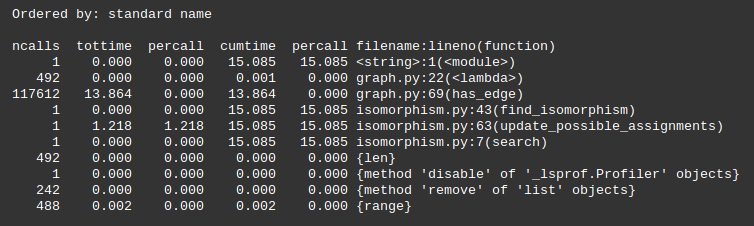
\includegraphics[scale=0.6]{images/perf}
    \caption{Sample run of the Python implementation of subgraph isomorphism.}
  \end{figure}

  \subsection{C++ Implementation}

\section{Conclusion}
  Over the coming two weeks, we should have completed the OpenMP parallelizations and thoroughly tested the performance of the resulting program.

\section{Appendix}
  \subsection{Python Code}
    \subsubsection{Graph Class}
      \lstinputlisting[language=Python,caption={Python graph class.}]{../../src/pythonvers/graph.py}
    \subsubsection{Subgraph Isomorphism Algorithm}
      \lstinputlisting[language=Python,caption={Python algorithm to find isomorphism.}]{../../src/pythonvers/isomorphism.py}
    \subsubsection{Main}
      \lstinputlisting[language=Python,caption={Python main function to process arguments and run the ismorphism algorithm.}]{../../src/pythonvers/main.py}

  \subsection{C++ Code}
    \subsubsection{Graph Class}
      \lstinputlisting[language=C++,caption={C++ graph class.}]{../../src/graph.cpp}
    \subsubsection{Subgraph Isomorphism Algorithm}
      \lstinputlisting[language=C++,caption={C++ algorithm to find isomorphism.}]{../../src/isomorphism.cpp}
    \subsubsection{Main}
      \lstinputlisting[language=C++,caption={C++ main function to process arguments and run the ismorphism algorithm.}]{../../src/main.cpp}

  \printbibliography[heading=bibintoc,
                     title={References}]

\end{document}
